\paragraph{Example 1: No arguments}
\begin{lstlisting}[language=Python]
from BNumMet.Visualizers.NonLinearVisualizer import NonLinearVisualizer
zerosVisualizer = NonLinearVisualizer()
zerosVisualizer.run()
\end{lstlisting}
\begin{enumerate}
    \item Initial State\\
    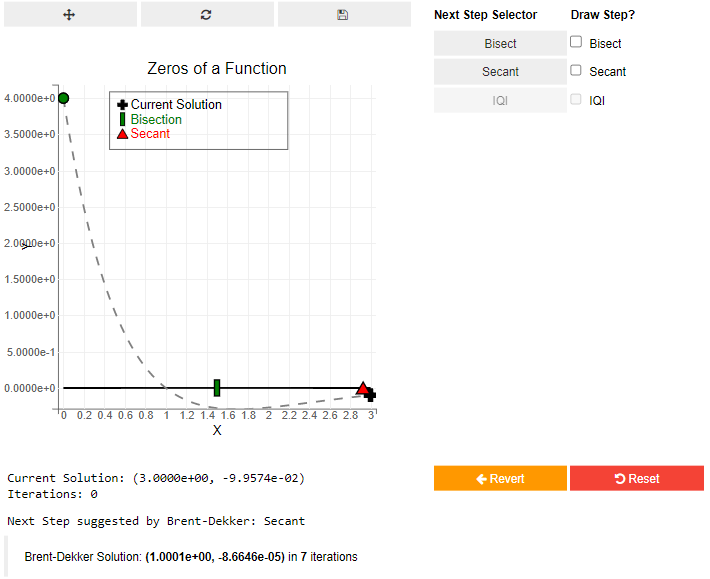
\includegraphics[scale=0.6]{Include/Images/Thesis/Documentation/Visualizers/NonLinear/Example 1/Example 1 - 00 - Initial State.png}
    \item Click on bisection checkbox\\
    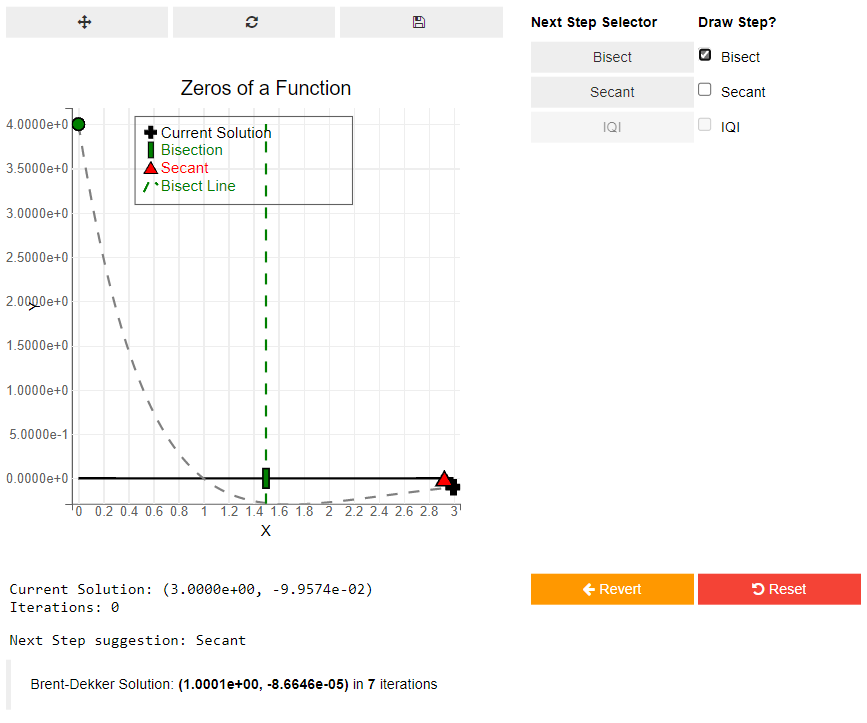
\includegraphics[scale=0.6]{Include/Images/Thesis/Documentation/Visualizers/NonLinear/Example 1/Example 1 - 01 - Bisection Checkbox.png}
    \item Click Secant Button\\
    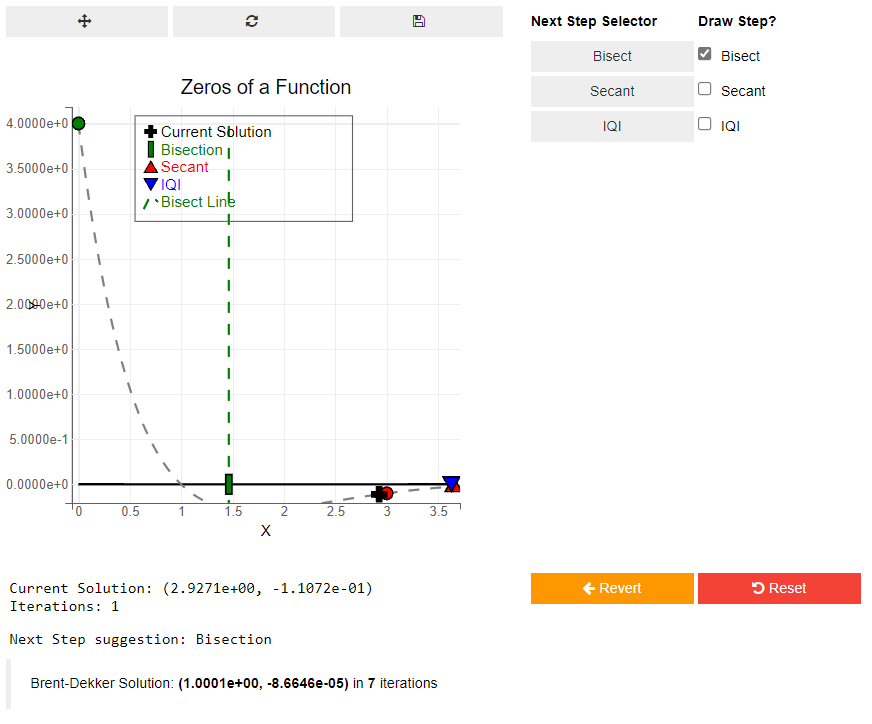
\includegraphics[scale=0.6]{Include/Images/Thesis/Documentation/Visualizers/NonLinear/Example 1/Example 1 - 02 - Click Secant.png}
    \item Some iterations after with secant checkbox clicked\\
    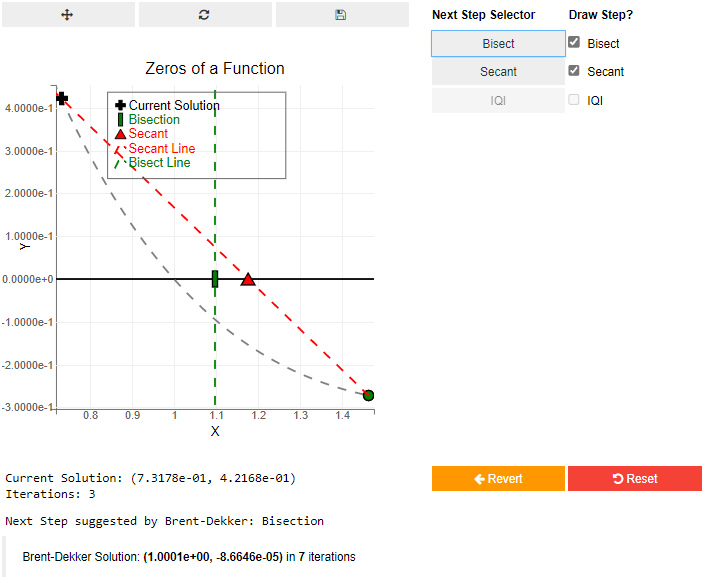
\includegraphics[scale=0.6]{Include/Images/Thesis/Documentation/Visualizers/NonLinear/Example 1/Example 1 - 03 - SOme iterations with secant checkbox.png}
    \item IQI Checkbox Only\\
    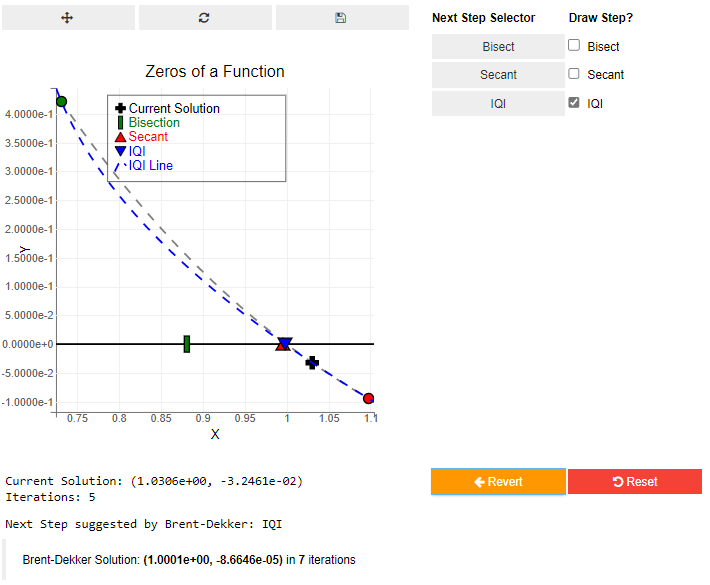
\includegraphics[scale=0.6]{Include/Images/Thesis/Documentation/Visualizers/NonLinear/Example 1/Example 1 - 04 - IQI checkbox only.png}
\end{enumerate}



\paragraph{Example 2: With Arguments}
\begin{lstlisting}[language=Python]
from BNumMet.Visualizers.NonLinearVisualizer import NonLinearVisualizer
f2 = lambda x: 0 if abs(x) < 3.8 * 10 ** (-4) else float(x * np.exp(-1 / x**2))
interval = (-1, 2)
zerosVisualizer = NonLinearVisualizer(f2,interval)
zerosVisualizer.run()
\end{lstlisting}

\begin{enumerate}
    \item Initial State\\
    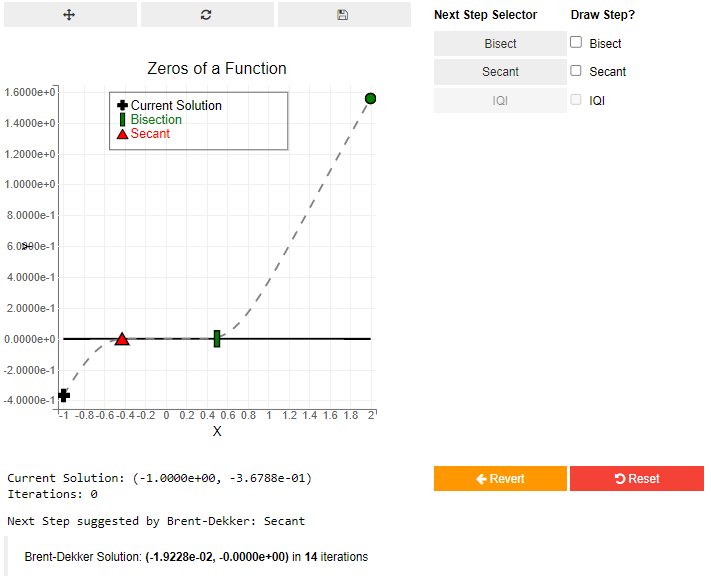
\includegraphics[scale=0.6]{Include/Images/Thesis/Documentation/Visualizers/NonLinear/Example 2/Example 2 - 00 - Initial State.png}
    \item All Checkboxes checked\\
    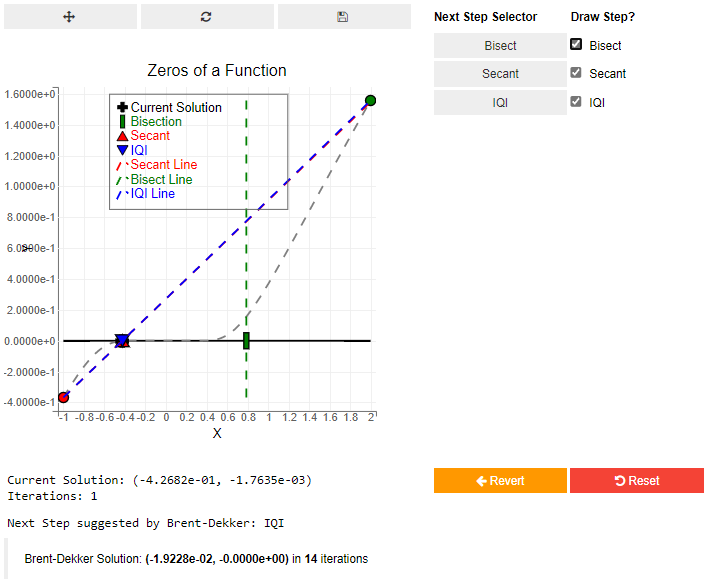
\includegraphics[scale=0.6]{Include/Images/Thesis/Documentation/Visualizers/NonLinear/Example 2/Example 2 - 01 - All Check Boxes.png}
    \item Click secant and click select all checkboxes again\\
    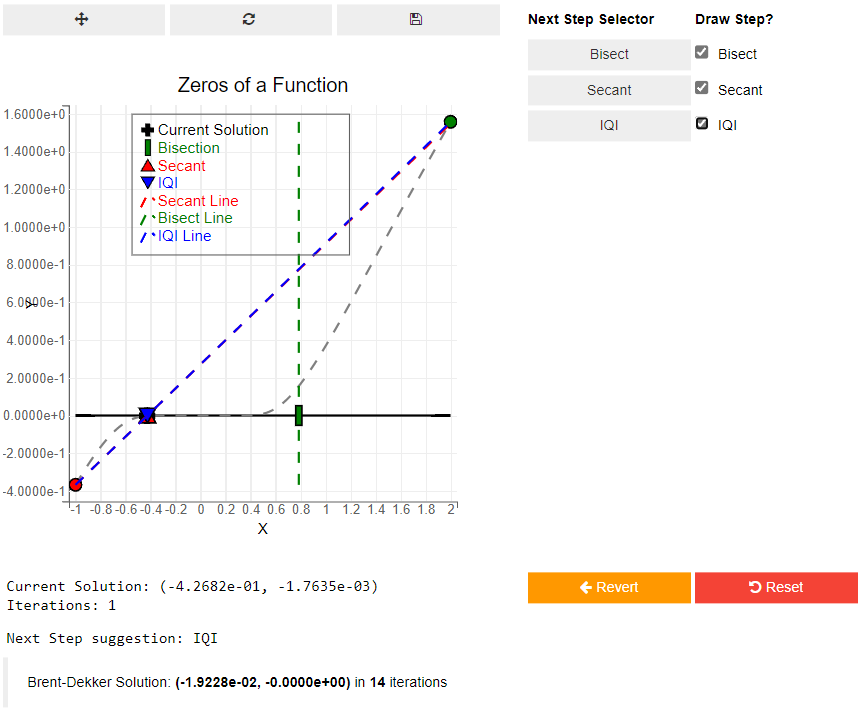
\includegraphics[scale=0.6]{Include/Images/Thesis/Documentation/Visualizers/NonLinear/Example 2/Example 2 - 02 - Click secant and All Check Boxes.png}
    \item Revert Button\\
    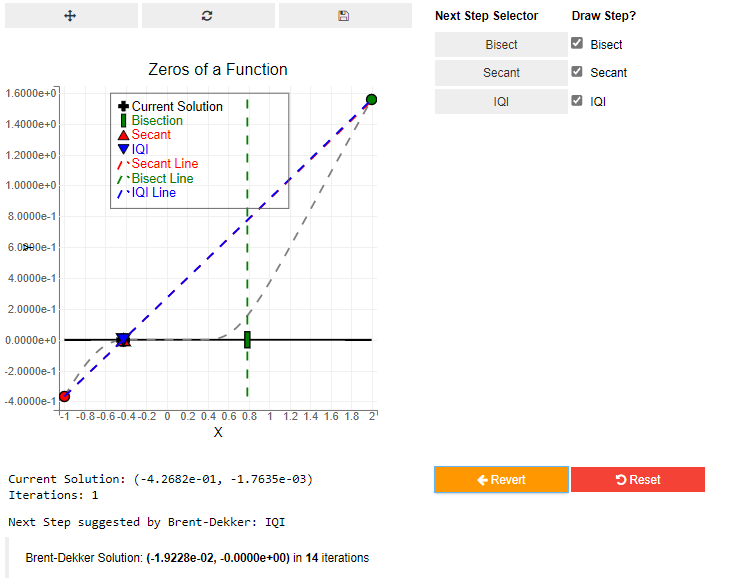
\includegraphics[scale=0.6]{Include/Images/Thesis/Documentation/Visualizers/NonLinear/Example 2/Example 2 - 03 - Revert Button.png}
    \item Some iterations\\
    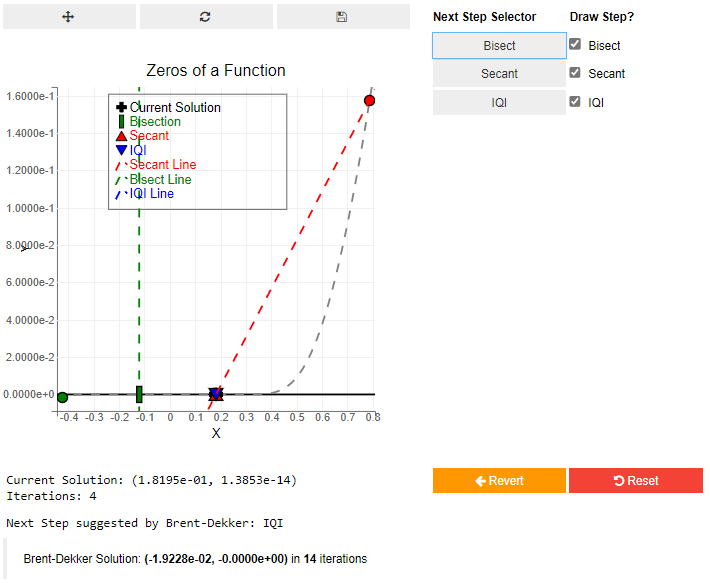
\includegraphics[scale=0.6]{Include/Images/Thesis/Documentation/Visualizers/NonLinear/Example 2/Example 2 - 04 - Some Iterations.png}
    \item Reset Button clicked\\
    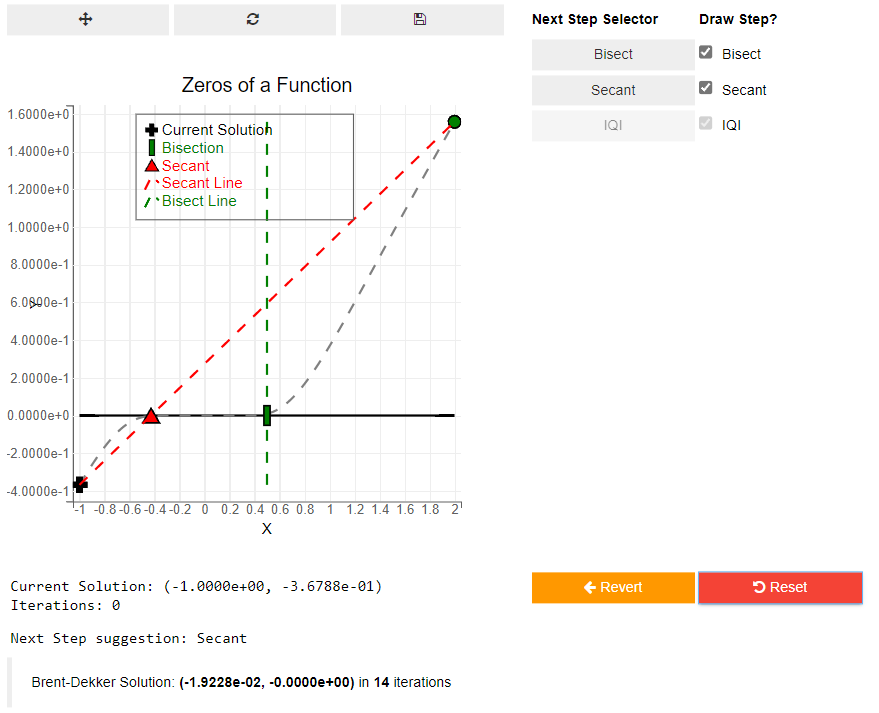
\includegraphics[scale=0.6]{Include/Images/Thesis/Documentation/Visualizers/NonLinear/Example 2/Example 2 - 04 - Reset Button.png}
\end{enumerate}